\section{Earlier empirical illustrations}\label{app:earlier-illustrations}
These experiments concern the earlier Harmonic implementation and seeded
finite-word decoder. The latter is not the finite-panel Taylor model
of \Cref{thm:compression}; none of the decoder measurements below validates
the new cubic-logarithmic theorem. We preserve the original measurements,
controls and failures without reinterpreting their scope. In this appendix,
$b_n(10^{-4})$ denotes the historical whole-sphere quantile
\begin{equation}
 b_n(10^{-4})=\inf\{b\ge0:\Pr(\norm{f_n-\widetilde f_n}_*\le b)\ge0.9999\}.
 \label{eq:intrinsic-benchmark}
\end{equation}
Here $\norm{\cdot}_*$ is the whole-sphere instance of
\eqref{eq:test-norm}, with discrepancy $+\infty$ on a run lacking a
required fitted limit. This quantile belongs to the supplementary seeded
decoder comparison, not the main theorem's negligible-relative-error claim.
The label
``Logarithmic'' inside the preserved figures refers to the seeded decoder.

\subsection{Trajectory fidelity and retained state}
\label{sec:experiments}
Earlier experiments test empirical Harmonic and seeded decoder implementations
against independent dense-run variability. Error is the largest unseen-input
RMS discrepancy at recorded common times; the practical threshold is three
times the corresponding dense-pair discrepancy, not the historical quantile
$b_n(10^{-4})$. Harmonic meets this threshold in all nine held-out circle cases
($n=1024,2048,4096$, three seeds), with ratios $0.159$--$1.617$.
At $n=4096$ it uses $11.7$--$11.8$ times fewer model-tensor scalars.
Single-seed checks in dimensions $3,5,10$ also meet the threshold.
On digits $3$ versus $8$, three width-$4096$ runs preserve the dense
teacher's $97.32\%$ accuracy with about $4.6$-fold smaller tensor state;
their fidelity ratios are $1.85$--$2.44$. The matched smaller networks
have better fidelity on all three real-data runs. Thus compression
success does not establish superiority over ordinary small networks.

The seeded decoder implementation retains $688{,}220$ numerical words across
the tested dimension-five widths $1024,2048,4096$, a $24.4$-fold persistent
payload reduction at width $4096$. All five dimension-five confirmation
cases meet the empirical threshold, with ratios $0.909$--$1.781$ against
independent dense references. Its circle check fails, with ratio $6.95$;
a separate digits decoder check also fails ($4.94$). These results are
not a universal success claim. \Cref{fig:compression-validation}
shows both state and fidelity comparisons. Full-horizon source construction
is charged as offline setup, so these experiments demonstrate no setup
speedup. The implementations, query workspace, numerical checks and negative
cases are detailed in \Cref{app:empirical}. Fresh labels have RMS one and need
not satisfy the small-label theorem. The earlier Legendre trajectory in
\Cref{fig:trajectory} remains a separate illustration.
\begin{figure}[t]
 \centering
 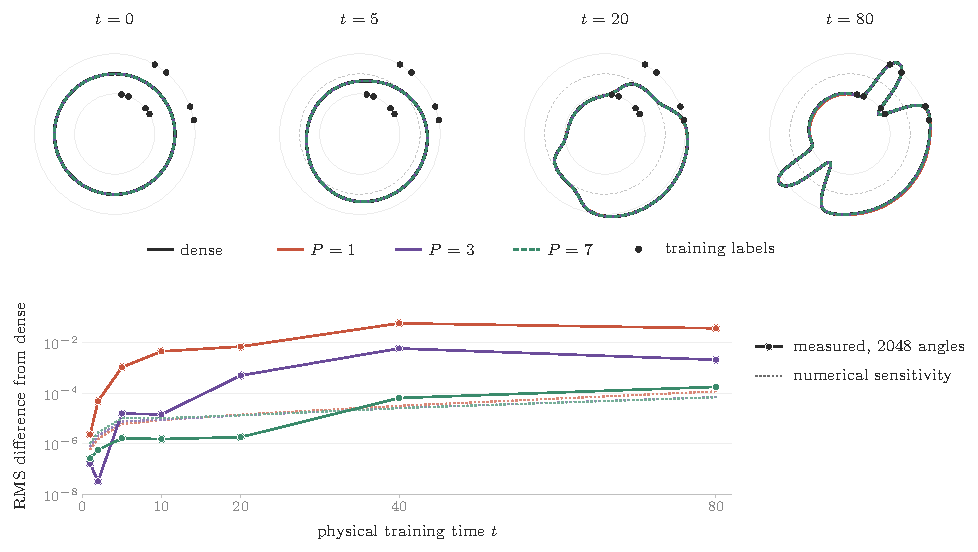
\includegraphics[width=\textwidth]{figures/trajectory.pdf}
 \caption{\textbf{A trajectory, not only an endpoint.}
 Existing paired-label circle experiment: two hidden tanh layers,
 width $2048$, and Legendre orders $q=1,3,7$. Predictions are saved at
 the same physical times $t=0,5,20,80$. Radius is $3+f(\theta)$, the
 dashed ring marks zero, and black points are training labels.
 The source replay records $39$ common times and uses float64 adaptive
 Heun integration at two tolerances. These are discrete observations,
 not a certificate between the saved times.}
 \label{fig:trajectory}
\end{figure}
\begin{figure}[t]
 \centering
 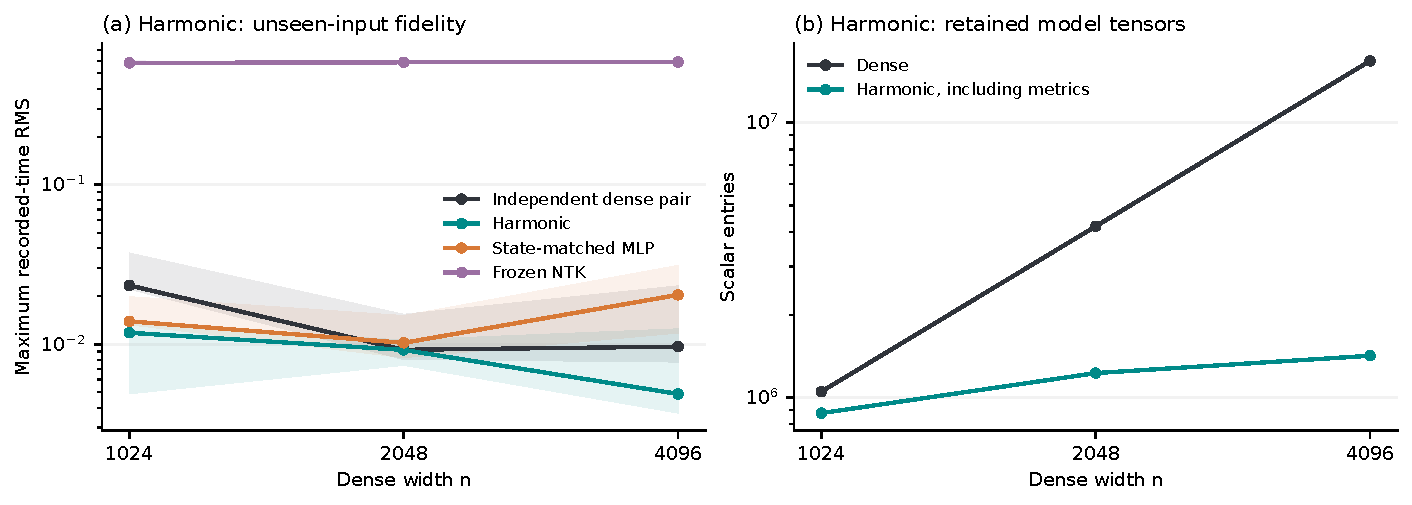
\includegraphics[width=\textwidth]{figures/compression_validation.pdf}
 \par\smallskip
 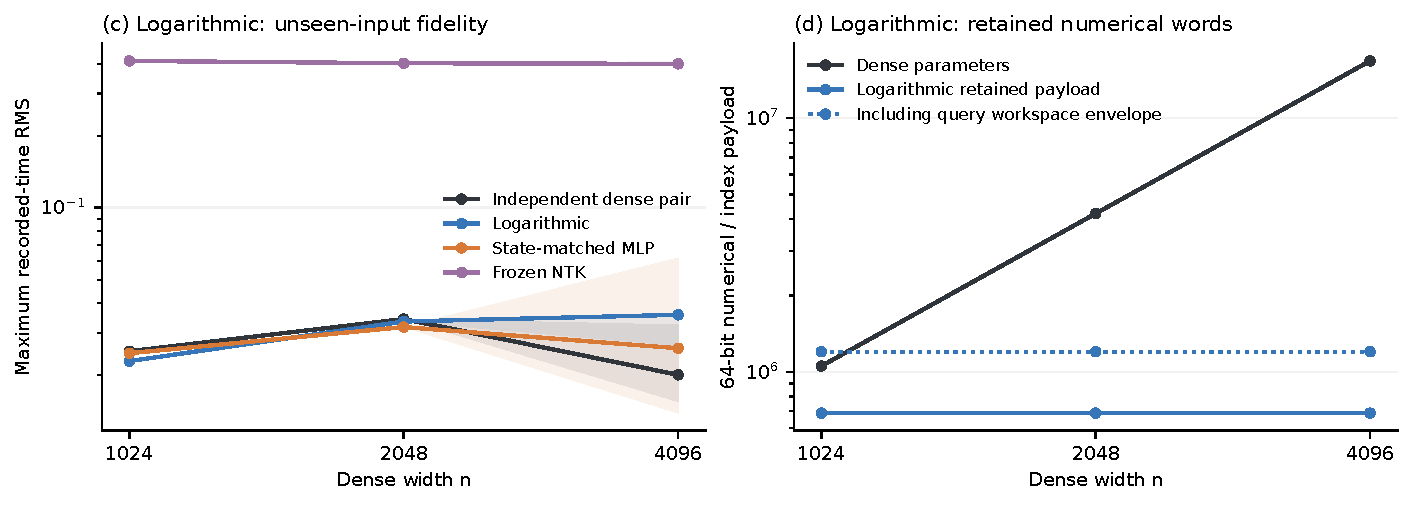
\includegraphics[width=\textwidth]{figures/compression_logarithmic.pdf}
 \caption{\textbf{Retained state and finite-time prediction fidelity.}
 Top: Harmonic circle confirmation, with three held-out seeds at each
 width and a coupled dense reference. Bottom: the dimension-five
 seeded decoder finite program, with seed 201 across widths and three
 seeds at width $4096$, compared with independent dense references.
 Ordinary small-network controls match retained payload; the frozen
 initial kernel uses the dense initialization and physical clock.
 Ratios use a measured dense pair on the same times and queries.
 Storage means model-tensor scalars for Harmonic and persistent
 numerical payload for seeded decoder; setup and query workspace are
 additional (the dotted curve includes the latter's numerical envelope).
 Lines show medians and shading shows the full observed seed range,
 not confidence intervals. The fixed finite program's flat payload across these
 widths is not an asymptotic scaling estimate.}
 \label{fig:compression-validation}
\end{figure}
\FloatBarrier

\subsection{Protocol and additional results}
\label{app:empirical}
\begingroup
\small
\paragraph{Observable and split.}
For recorded physical times $\mathcal T$ and unseen inputs $\mathcal Q$, use
\[
 E(g,h)=\max_{t\in\mathcal T}
 \left(\frac1{|\mathcal Q|}\sum_{x\in\mathcal Q}
 |g(t,x)-h(t,x)|^2\right)^{1/2},\qquad
 R_{\rm emp}=\frac{E(f_{\rm model},f_{\rm reference})}
 {E(f_n,\widetilde f_n)}.
\]
The denominator uses independent dense initializations. A practical pass
requires $R_{\rm emp}\le3$ and resolved reference numerics; Harmonic's
combined coarse--fine sensitivity must also be at most $10\%$ of that
denominator. This is neither a confidence estimate for $b_n(10^{-4})$ nor a
continuous-time, whole-sphere or asymptotic guarantee. Pilots use seeds
101--102; settings were frozen before seeds 201--203. Setup nodes are
separate from test queries. Digits uses 32 training images, training-only
PCA to dimension eight, normalization to unit directions, 64 tuning images
and 261 held-out images.

\paragraph{Dynamics and empirical backends.}
All runs in this experiment use two tanh hidden layers, zero readout, Gaussian
initialization and mobilities $(n,1,n)$ from \Cref{eq:dense-flow}; stored
inputs are $v=x/\sqrt d$. Labels have RMS one. Harmonic and dense use
float64 RK4, with steps $0.125$ and $0.0625$, through time 20. Harmonic's
full dense warmup is followed by Chebyshev/sphere-polynomial least squares
and per-family SVD truncation before paired mixer images are formed.
Mandatory initialization fields, BSS selection, full metrics and the
corrected optimizer are retained. The circle uses family rank
$\lceil2\log(en)\rceil$, time degree five and circle degree nine;
dimension checks use rank $\lceil\log(en)\rceil$ and degrees three.
Digits uses rank 19. These source approximations have no certified
uniform error bound. All use nine time nodes; the circle, sphere checks
and digits use respectively 64, 128 and 256 passive spatial nodes.
The toy circle has seven training points and target
$\sin(3\theta)+\tfrac12\cos(5\theta)$; the sphere target on unit
directions $v$ is $\sqrt d\,v_1+d^{3/2}v_1v_2v_3$.
Training-label RMS normalizes the targets. Harmonic uses 256 test directions,
twelve sphere training points, and times $0,0.5,1,2,5,10,20$.
seeded decoder uses ten Euler panels of length $0.5$,
noise $0.01$, one member and 32 queries through time five. It retains
both Gaussian orientations and covariance corrections, immutable row
fields, causal metric replay and empirical query sums. Float64, a
conventional counter PRNG and numerical-rank selection replace the
certified finite-word backend; no bit, PRG or confidence certificate
is asserted. Its fixed Euler program is not an integration-convergence
study. Toy decoder checks use $m=\max(d,3)$ and the common recorded times
$0,0.5,1,2,5$. Harmonic is coupled to its source; the decoder's target is independent.

\paragraph{Controls, storage and costs.}
Small MLPs train all layers at the same canonical mobilities, with width
chosen to fit the retained payload. At zero readout, the exact frozen
initial NTK has only its readout block; its constant-kernel flow is solved
spectrally without ridge or time rescaling. Harmonic counts
$q_1d+q_1q_2+q_2+m$ moving and $2q_1^2+q_2^2$ fixed tensor scalars.
Common training data, measurement copies and query scratch are separate.
seeded decoder counts data, seeds, selected fields, metric caches, acquired
pairs, field instructions and immutable coefficients as 64-bit payload;
Python overhead is excluded. In dimension five its retained-plus-batched-query
workspace envelope is $1{,}201{,}027$ words: about $14.0$-fold smaller
than the width-$4096$ dense parameters, but larger than the width-$1024$
dense parameters. Source setup, training, readout refresh and batched
queries are timed separately. Runs use two RTX 3090 GPUs and CPU scalar
programs, with 120-second toy and at most 300-second real-data model caps.
These measurements establish no end-to-end speedup.

One circle confirmation also compares explicit LoRA increments with trained
outer layers at width $2048$. Its $313{,}344$ moving scalars match Harmonic's
$315{,}481$ from below, but its $4{,}194{,}304$ fixed mixer scalars are additional.
Orthonormal initial right factors and zero left factors preserve the dense
initialization. The factor mobility multiplier $0.25$ was selected from
$0.25,1,4$ on pilot seed 101; steps $0.01$ and $0.005$ resolve the held-out
seed-201 comparison. LoRA's discrepancy is $7.51$ dense-pair units versus
$0.479$ for Harmonic. This is evidence against this matched-moving-state
factorization and optimizer, not against every low-rank alternative.

For timing context, the width-$4096$ circle seed-201 Harmonic source rollout
and spectral fit take $4.75$ seconds, followed by $4.96$ seconds of assembly.
Its RK4 updates take $12.5$ ms per step versus $27.7$ ms for dense, at step
$0.125$; these figures exclude query evaluation and the separate refinement.
For dimension-five seeded decoder seed 201 at the same width, CPU source and
metric setup take $0.66+0.84$ seconds, ten causal training panels take $0.46$
seconds, and all five batches of 32 passive queries take $3.31$ seconds.
The tasks, clocks, solvers and hardware differ, so these are separate measured
costs, not a cross-method speedup ratio. Device peaks in the records include
other resident references; payload counts are not isolated process-RAM peaks.

\paragraph{Additional and negative results.}
Harmonic's dimension-$3,5,10$ ratios are $0.751,0.937,0.997$ at width
$2048$ (one seed each). The real-data smaller-MLP ratios are
$0.646$--$1.123$, below Harmonic's $1.85$--$2.44$; one also attains
$97.70\%$ accuracy. The frozen-kernel circle ratios are $15.6$--$76.6$,
so the measured trajectories depart substantially from that control.
seeded decoder's width-$4096$ dimension-three and dimension-ten checks
give $1.84$ and $1.26$, while the circle gives $6.95$ and fails.
A dimension-ten pilot with twenty Euler panels exceeded the 120-second
cap; the ten-panel pilot passed before its rule was frozen.
A separate digits decoder experiment uses eight training images, training-only
PCA dimension five and all 285 held-out images. The twenty-panel setting
passed its tuning split but fails the single held-out confirmation:
$R_{\rm emp}=4.94$, versus $3.02$ for its payload-matched MLP. The decoder
retains $6{,}608{,}623$ words ($2.54$ times fewer than dense), and its
retained-plus-batched-query envelope is $11{,}052{,}846$ words. Setup, replay
and queries take $67.9$ seconds in total. This is not the 32-training-image
Harmonic task and does not establish real-data decoder comparability.
\Cref{fig:compression-checks} retains these scope distinctions.
Gradient, metric, paired-action, posterior, replay and passive-query
checks precede evaluation. The full-retention Harmonic trajectory error
decreases approximately sixteenfold under RK4 step halving.
Commands, hashes, inventories and failures are retained in
\texttt{paper/figures/capture\_trajectory.py} and the study records under
\texttt{data/generated/compression\_empirical\_validation\_20261007/}.
\endgroup

\begin{figure}[p]
 \centering
 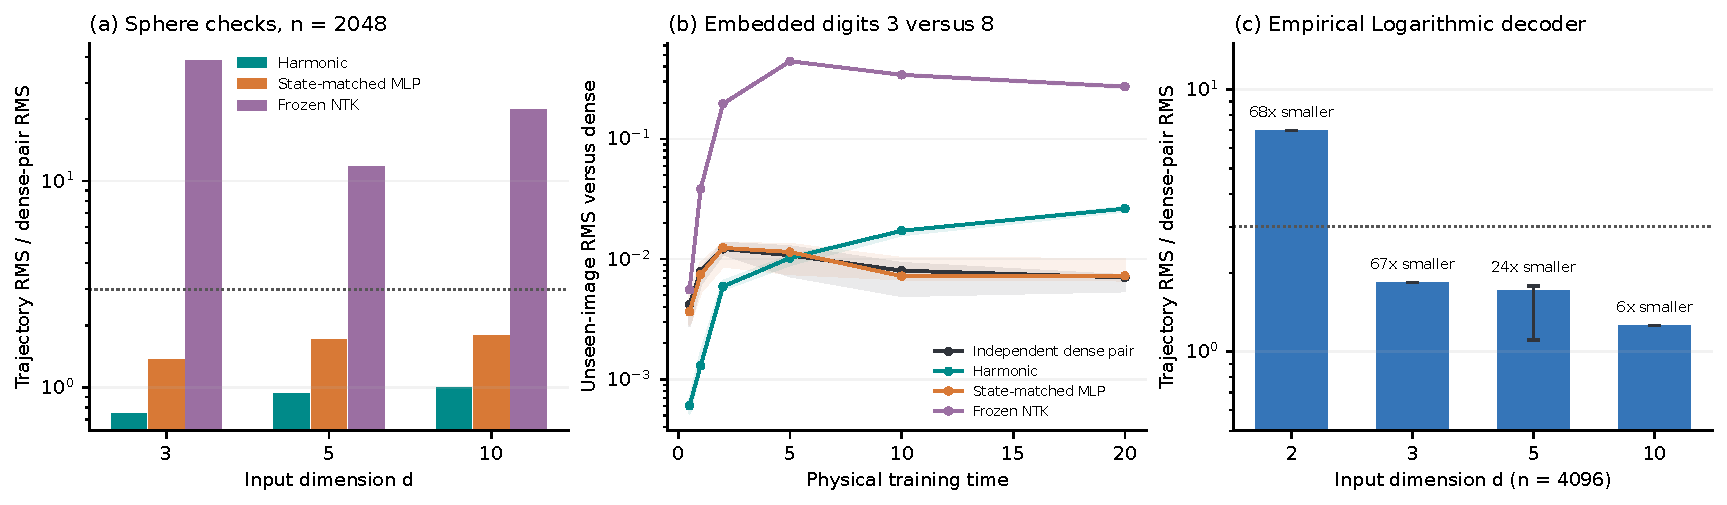
\includegraphics[width=\textwidth,height=.29\textheight,keepaspectratio]{figures/compression_checks.pdf}
 \caption{\textbf{Dimension, real-data and decoder checks.}
 Additional finite-time comparisons supplement the width experiments.
 Dimension checks use one held-out seed; digits uses three.
 The dimension-five decoder bar summarizes three seeds, the others one;
 its annotations count persistent payload only, excluding query workspace.
 Lines/bars show medians and ranges show all observed seeds.
 The empirical factor-three threshold is not a confidence statement.
 The circle decoder failure and matched small-network controls prevent
 interpreting the favorable cases as uniform superiority.}
 \label{fig:compression-checks}
\end{figure}
\begin{figure}[p]
 \centering
 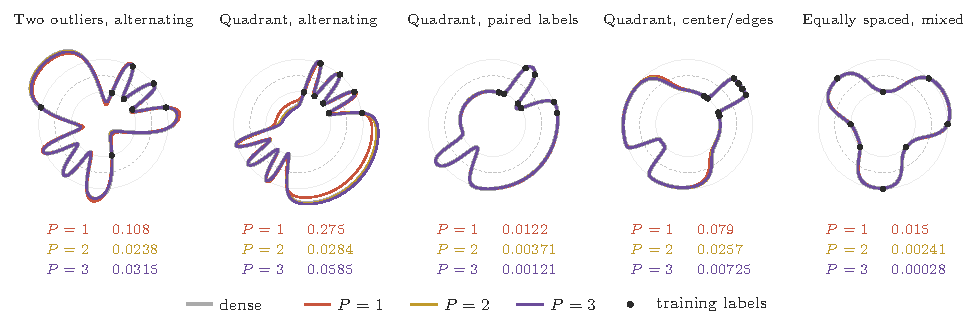
\includegraphics[width=\textwidth,height=.29\textheight,keepaspectratio]{figures/circles_deep.pdf}
 \caption{\textbf{Earlier Legendre fitted-function illustration.}
 Existing five-task comparison: three hidden tanh layers, width $4096$,
 and Legendre orders $q=1,2,3$, at each model's own training-MSE
 $10^{-3}$ endpoint, not a shared time. Grey curves are dense predictions,
 coloured curves are memory predictions, and black points are labels.
 Printed discrepancies are RMS differences on $8192$ circle queries,
 not uniform errors or risk against unseen labels. Fixed initialized
 matrices remain additional to Legendre's moving state. This archived
 illustration is separate from the earlier confirmation runs above.}
 \label{fig:deep}
\end{figure}
\FloatBarrier
\clearpage
